\chapter{Contribuição}\label{meto}

A contribuição dessa pesquisa é de cunho metodológico-prático.
Do ponto de vista metodológico pela aplicação do processo CRISP-DM, usado para construir o modelo preditivo e classificativo; do ponto de vista prático pela proposição de um modelo que integre predição à API de mapas de posicionamento global, fornecendo informação suficiente a um gestor para decidir quando e por onde enviar uma carga por determinada rodovia que apresente retenções crescentes de logística de cargas. 

As soluções disponíveis que existem tais como; Google Maps, Waze e outros dessa natureza somente exibem informações momentâneas, produzidas e compartilhadas pelos utilizadores dos aplicativos ou por informações provindas de GPS, contudo não analisam dados históricos dessas rodovias nem fazem predições sobre o seu comportamento.

Outra contribuição dessa pesquisa é a proposição de um arco cibernético construído com a API de redes sociais.
Os ``feeds'' de notícias das redes sociais como o Twitter permitem analisar o contexto das rodovias com defasagem temporal muito pequena.
Os utilizadores dessas redes sociais contribuem com muita informação relevante como por exemplo o anúncio de uma paralisação que ocorrerá 
daqui a uma semana, a PRF de Pernambuco é outro contribuidor permanente; com seu canal no Twitter: @PRF191PE fornece diariamente informação das rodovias 
além de dados estatísticos. 

A monitoração de redes sociais é feita por Mineração de dados em textos conhecida como "Text Mining" (TM).
A TM a princípio foi executa somente no Twitter no canal PRF191PE. Agentes da PRF disseram que os protestos quando feitos dentro da lei
devem ser informados à PRF, com dia e hora marcados antecipadamente.
Para ter-se acesso aos twittes postados da PRF os usuários do canal, inclusive a própria PRF, postam comentários diretamente 
por um navegador Twitter palavras chaves tais como: protestos, acidentes, paralisação.  a API do 

Uma vez capturadas e tratadas as informações desses ``feeds'' são analisados instantaneamente por algoritmos de I.A. 
A técnica utilizada é o Processamento de Linguagem Natural (PLN). O algoritmo escolhido foi Naive Bayes por ser um classificador 
rápido e eficiente e por ter sido utilizado na primeira fase em que foi como comparativo à Árvore de Decisão de simples implementação 
poderão ser direcionadas a um banco de dados para o caso de novos estudos.



\section{Modelo Proposto}

A metodologia utilizada nessa pesquisa contempla um plano em três etapas, cada uma dividida em fases atinentes.
A primeira etapa da nossa metodologia completa o ciclo todo do processo CRISP-DM, onde está o modelo preditivo e 
a descoberta de conhecimento sobre o comportamento das rodovias estudadas. A descoberta de conhecimento sobre esses comportamento 
nas rodovias tem a ver com o ``modus operandi'' dos utilizadores. A priori especulou-se sobre possíveis erros de traçados e outros que possam
ser identificados pelos algoritmos de mineração empregados no processo.

Os algoritmos escolhidos contemplaram algumas características especiais, tais como; robustez, tolerância à faltas (missing data),
taxa de aprendizagem, e facilidade de interpretação dos dados processados. 

No quesito tolerância à falas e facilidade de interpretação dos dados a Árvore de Decisão e o Naïve Bayes se destacaram por não necessitar
de nenhum requisito extra para entender e interpretar os resultados[referencia].

No quesito robustez, tolerância à faltas e taxa de aprendizagem relativamente alta, as redes neurais artificiais (RNA), com a 
topologia Perceptron multicamadas com retroalimentação ``backpropagation'' se destacaram. 
As redes neurais têm capacidade de generalização e especificidade em modelos de previsão[referencia]. 

A extrapolação do modelo preditivo ocorre quando este se integra à uma estrutura dinâmica a serem exibidas em mapas vetoriais, 
dado um espaço temporal pré-determinado por um agente; o utilizador. 
Através de API's os mapas vetoriais permitem a geolocalização dos pontos classificados ou os pontos onde haverá grande número de 
retenções, conhecido no meio da logística de cargas como \textbf{gargalo}.
A API do Google-Maps é o ``front end'', foi escolhida por permitir maior pela portabilidade e simplicidade para integração da estrutura
dinâmica com a preditiva.

Para a integração às redes sociais, foi escolhida a API do Twitter. Esta ``interface'' é simples de ser configurada e gera poucos dados; 
o utilizador tem que ser eficaz ao publicar suas postagem em um espaço de 140 caracteres, isso facilita a forma como os dados são
extraídos pela quantidade diminuta deles, bem como a quantidade conexões à Internet, contudo está rede social tem uma crescente quantidade
de postagens no formato imagens, isso dificulta a mineração em textos.
A API do Twitter tem a finalidade de integrar o modelo dinâmica dos mapas vetoriais às redes sociais. 
Esta ``interface'' é responsável por fornecer ``input'' à terceira etapa, servindo de ``busca local'' das informações mais recentes das 
redes sociais, relativas à trechos das rodovias; os ``feeds'' do Twitter (ou twetts) fornecem dados que serão minerados e interpretados à posteriori.

A figura a seguir ilustra (um overview) essa metodologia descrita graficamente.

\pagebreak

\begin{figure}[ht]
\centering
\caption{Etapas da modelo proposto}
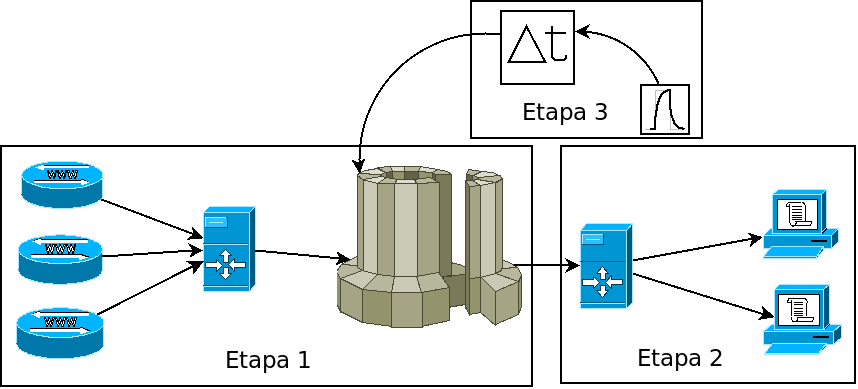
\includegraphics[width=170mm, height=85mm]{Figuras/Metodologia/metodologiaGeral.png}\\
\tiny Fonte: autor
\end{figure}

\section{Reflexão sobre as tecnologias utilizadas no modelo preditivo}\label{result}

As técnicas preditivas tradicionais que contemplam análise de grandes massas de dados como base homogêneas.
Não existe uma técnica de mineração que generalize os mais diversos ambientes preditivos, mas sim um ``pool'' 
dessas técnicas onde uma complementa outra como identificamos nos artigos de ZENG, HUANG, PEI \textit{et al} (2016), 
POSSAS, BAV e CARVALHO (1998), e BESHAS e HILL (2010).



são possíveis quando adaptadas para uma forma comparável à que
foram inicialmente concebidas, por que as variáveis em uma base de dados a priori guardam pouca relação as variáveis de outra base de dados.
neste caso essas variáveis ou são excluídas ou são transformadas a fim de ``guardarem'' um correlação com a outra base de dados. 

Na fase de transformação de dados, da primeira etapa, onde são criadas novas variáveis, a proximidade entre as
bases heterogêneas foi conseguido utilizando de regras de indução da lógica proposicional \cite{NorvigRussel2004}.
Nesta pesquisa, bases heterogêneas foram integralizadas num única grande conjunto de dados o ``data set''. As variáveis desse ``data set''
são consideradas variáveis independentes, foram preservadas as com maior relevância ou as que continham a maior quantidade de conhecimento
embutido.  construídas novas, nas bases onde não haviam correspondência, respeitando a lógica do negócio.\\
A tabela a seguir descreve as variáveis originais na base de dados de acidentes da PRF 

\pagebreak

\section{Extração do conhecimento - KDD}

O processo de descoberta do conhecimento iniciou-se com a coleta das bases de dados de acidentes da PRF. Optamos por coletar os dados dessa base diretamente na fonte,
ou seja dos servidores da PRF. Esses dados nos foram cedidos após alguns procedimento burocráticos de praxe (ver anexos). Essa escolha foi motivada para tentar
mitigar o problema da qualidade dos dados. No artigo ``Uma análise da qualidade dos dados relativos aos boletins de ocorrências das rodovias 
federais para o processo de Mineração de Dados'' COSTA, BERNARDINI, LIMA et al (2012) destacam a não padronização e não aceitação dos dados pela 
comunidade internacional. EAVES, D. (2009) sugere que os dados sejam disponibilizados na maneira como foram coletados.

A PRF tem ao menos duas bases \footnote{Somente mencionamos bases de dados que foram interessantes à essa pesquisa.} de dados referentes às ocorrências 
nas rodovias BRs. A base de acidentes rodoviários e a base de intervenções que ``guarda as ocorrências que paralisaram as rodovias, tais como:
protestos ou paralisações dessa natureza, feitos pelas pessoas que vivem no entorno dessas rodovias.

As técnicas como Redes Neurais Artificias (MLP) \cite{DecisaoCredito}, Árvores de decisão (CART) \cite{DataMining}, Regressão logística (MLR) 
\cite{RegrecaoLog} fornecem visão generalizada dos fatores preponderantes, levantando padrões ocultos nos dados. Esta fase é conhecida como 
Aprendizagem de Máquina (acrônimo de Machine Learning)

\begin{itemize}
 \item[a] Redes Neurais Artificias do tipo \textit{ Multi Layer Perceptron}  -- (MLP) têm capacidade de receber várias entradas ao mesmo tempo e distribuí-las de maneira organizada, além 
	  são simples de implementar e trazem resultados satisfatórios em grandes bases de dados.
 
 \item[b] Árvores de decisão do tipo \textit{ Classification and Regression Tree}  -- (CART) foi empregue por Pakgohar et al no artigo 
	  \textit{The role of human factor in incident and severity of road crashes based on the CART and LR regression a data mining approach}  para classificar acidentes 
	  com nível de acurácia próximo aos 80\%

 \item[c] Regressão logística tipo \textit{Multinomial Logistic Regression} -- (MLR) fornece a possibilidade de aprofundamento em vários níveis de busca sendo a mais apropriada, já que Regressão logística 
	  tradicional não permite aprofundamento desse tipo no espaço de busca.
\end{itemize}



\section{Reflexão sobre as tecnologias utilizadas no modelo preditivo a posteriori}\label{resultPost}


(Artigo ``Library \& Information Science Research'')
Tecnologia
Para encaminhar as pesquisas, os autores usaram uma abordagem indutiva. Os mais recentes 1200 tweets foram coletados da conta (Tweet de uma Universidade) de todos os membros da Association of American Universities (AAU). Os dados foram coletados e processados usando o Twitter API com o twitter4j (biblioteca Java) e adicionados a um código java desenvolvido pelo autor. ...Foi reduzido a uma amostra do percentual da academia….
Os dados coletados foram preprocessados para preparar a analise. Retweets foram removidos das amostras. Em seguida tweets com pouco conteúdo foram removidos, tal como breves agradecimentos (e.g. “welcome”) breves comentários de algum tweet (e.g. “lol”) pequenos encorajamentos (e.g. “keep going”) e conversas pessoais foram removidas das amostras. Isto reduziu a amostra de 1200 para 752 tweets. Estes tweets foram em seguida categorizados em nove categorias…
Dos 752 tweets analisados, 271 tinham ao menos um retweet e 131 receberam um “favorito”. Em média, tweets recebidos 0,67 (desvio padrão “SD” = 1,4) retweets e 0,23 (SD=0,6) favoritos. Adicionalmente, em média, tweets incluídos 0,47 (SD=0,51) URLs, 0,61 (SD=0,91) menções de usuários e 0,04 (SD=0,2) media de entidades. Em média o tamanho dos tweets foi 107 (SD=29,81) caracteres.
Na média, as seis contas de Twitter das bibliotecas analisadas enviaram 1817 (SD=1126) tweets, seguido 1062 (SD=641) usuários, estes seguidos por 2006 (SD=788) usuários, e estes 1503 (SD=450) dias (duração). O teste Shapiro-Wilk mostrou que nove característica de tweets normalmente distribuídas. Consequentemente métodos não paramétricos foram usados para examinar a relação entre um tweet  as características da conta.
O teste Kruskal-Walls revelou uma diferença estatística significativa entre o conteúdo da categoria do tweet para o número de favoritos (X² = 15.11, df =8, p < 0,057).
O teste Spearman mostrou uma correlação negativa entre o número de retweets e o número de menções a usuários. Isso sugere que tweets com conexões pessoais podem ter pouco valor de ‘uso geral’ e esses usuários podem estar relutantes em retweetar o conteúdo desses seguidores.
O teste Spearman encontrou uma pequena correlação positiva entre o número de favoritos e o número de usuários seguidos, e encontrou uma baixa correlação negativa entre o número de favoritos e tempo de uso da conta (desde o cadastro).

(Artigo “A Text Mining Analysis of Academic Libraries Tweets”)
Análise de textos
Em mídias sociais, analisar o conteúdo e minerar textos é frequentemente usado para analise texto de usuários geral e suporte para tomada de decisão (Abrahams, Fan, Wang, Zhang \& Jiao, 2015). Aplicar mineração de textos em bibliotecas e outras instituições inclui extrair informações, rastrear tópicos, sumarização, categorização, agrupamento, ligar conceitos, visualização de informação e perguntas de questionários (Fan, Wallace, Rich e Zhang, 2006). De acordo com Zhang e Gu (2011) as bibliotecas acadêmicas poderiam utilizar mineração de textos para beneficiar os aplicativos no objetivo de suporte a tomada de decisões.
No recente artigo, Sandhu (2015) indicou a importância do aprendizado sobre mineração de dados e  ferramentas de Big Data para as bibliotecas acadêmicas para melhorar a eficiência da biblioteca e os serviços de informação. Similarmente Zhang e Gu (2011) alegaram que  minerar conhecimento sobre os clientes é importante para as bibliotecas acadêmicas. 
A abordagem de mineração de textos para os dados das mídias sociais tem sido utilizados em muitos outros campos, como negócios (business) (Abraham et al., 2015), ciência da saúde (Sarker et al., 2015) ciência política (Stieglitz \& Dang-Xuan, 2013).
O uso da abordagem de mineração de textos está lentamente começando a ser aplicada na literatura sobre biblioteca e Ciência da Informação…
Papatheodorou, Kapidakis, Sfakakis e Vassiliou (2003) estudaram o uso das técnicas de mineração para analisar o uso das comunidades digitais.
Zang e Gu escreveu um artigo sobre aplicação de “text mining” nos dados das vidas sociais.
Shulman et al. (2015) analisou a rede de Twitter em duas bibliotecas acadêmicas os esforços para identificar a influência dos “players” e o recrutamento deles para fins de disseminar informações.


Conjunto de Dados
O conjunto de dados desta pesquisa foram coletados completamente da “timeline” de 10 bibliotecas acadêmicas (i.e. todos Twittes desde a adesão à plataforma) através de um serviço de arquivamento (twimemachine.com) em dezembro de 2014. 
<<<<  Interessante essa ferramenta, instalei e pode ser usada para fazer mineração em textos  >>>>
As bibliotecas escolhidas foram as 10 maiores ranqueadas pelo Shanghai Ranking. A seleção foi restringidas para universidades que “falavam inglês” e a uma biblioteca se a universidade tinha mais que uma (no artigo original é a tabela 1). Adicionalmente para o conteúdo do tweet, as seguintes informações foram recuperadas: 
Data do tweet – “tweet date”,
Número de vezes marcados como favorito – “number of times marked as a “favorite” by other users”, 
Número de vezes retweetado “number of times “retweeted” e, 
Data que se “juntou” (entrou) ao Twitter.


Preprocessamento do conjunto de dados – ``dataset preprocessing''
O ``dataset'' recuperado foi ``limpo'' para reduzir os ruídos seguindo uma abordagem consistente com outros estudos de mineração (em textos) tal como Ralston, O’Neil, Wigmore e Harrison (2014) e Yoon, Elhadad e Bakken (2013). O passo-a-passo incluiu a aplicação de um número de filtros; por exemplo, foram removidas as ``stopwords''; pontuação e numeração, 
todos os nomes de usuários seguido por um símbolo ``@'', ``hashtags'' após o símbolo ``\#'' e ``hyperlinks'' após o ``http''. 
Também foi removido a abreviação do Twitter tal como ``RT'' (retweetes), e ``MT'' (tweet modificado), e palavras tal como ``via''. 
O nome do usuário do Twitter para cada biblioteca acadêmica também foi excluído.


Analise do Conjunto de dados – ``Dataset''
Mineração em textos e técnicas de análise de conteúdo foram usadas para analisar os históricos de tweets da bibliotecas. A frequência dos tweets, retweets e distribuição dos tweets e retweets o tempo todo foi identificado e “plotado”. Então os tweets foram limpos, abertos e marcados com o PamTaT, uma ferramenta “text mining” desenvolvida por Pamplin Collage do Instituto Politécnico de Negócios da Virgínia da(ligado à) Universidade Estadual de Virgínia.
PamTaT é baseado interface do Microsof Excel para Python nltk – “natural language processing framework” (Bird, Loper \& Klien, 2009).
PamTaT permite que grande volumes de textos sejam analisado pelos usuários finais sem requer conhecimento de programação da linguagem Python. Em particular foi usado PamTaT para determinar a frequência de palavras simples (unigramas), de duas palavras (bigramas) e sequencias de três palavras (trigramas) que aparecem no texto fonte. 
Isso permite-nos desenvolver uma matriz de frequência de termos-tweet mostrando como sequências de palavras simples e múltiplas palavras (n-grams) são usadas pela biblioteca acadêmica selecionada.
Adicionalmente “correu-se” com o Harvard General Inquirer (Stone et al. 1966) para análise semântica e sentimental dos tweets.  “Harvard General Inquirer” é uma ferramenta de análise de textos de propósito geral, esta permite ao usuário final repostar com que frequentemente categoria de palavras diferentes usadas no texto fonte. 
Aplicações reportadas no “General Inquirer” para diferentes textos fontes identificou (categoria) duas centenas de palavras incluindo, por exemplo: como positivo, negativo, relacionadas a vontade (prazer), relacionadas a dor, relacionadas a localização, relacionadas a hora (tempo), relacionadas a academia, relacionadas a exagero (overstatement) ou subavaliação (understatement) e assim por diante.
Hurtwitz (2002) forneceu uma lista abrangente de categorias de palavras reconhecidas pela  Harvard General Inquirer e proveu uma lista completa de palavras específicas que pertencem a cada categoria de palavras. No estudo desse artigo foi usou-se o  Harvard General Inquirer para determinar o número de palavras em cada categoria de palavras usadas em cada biblioteca.

-----------------

\pagebreak

\section{Arco cibernético com dados do Twitter}

Os dados do Twitter, permite uma busca imediata por novas informações que poderão ser confrontadas com o 
modelo preditivo aumentando o nível de confiança deste, com isso a informação construirá um Arco cibernético, que segundo Wiener (1948) a 
informação permite realimentação aos sistemas, com controle mais eficaz, por exemplo: no trecho da Br 101, na altura do km 5, no 
Município de Goiana alguém publicou que a comunidade que mora no entorno dessa localidade fará um protesto daqui a dois dias devido ao 
acidente ocorrido ou a PRF publicou que o km 80 da Br 232, na altura do Município de Gravatá será interditada amanhã, por 2h, para 
remoção/explosão de rochas. 
Essas informações, por serem a posteriori às predições, podem aumentar o nível de confiança sugerida pelo modelo preditivo e controle por 
parte do utilizador e dentro de um universo temporal mais restrito servir de comprovação do das predições.

No entanto pode ocorrer o contrário quando as informações provenientes do modelo de predição entrar em conflito com as informações 
provenientes das redes sociais \footnote{O sistema de predição é baseado em cálculos probabilísticos}, para estes casos a decisão de 
qual ação a ser tomada sempre estará ``nas mãos'' do agente, o observador ou o utilizador.

As informações das redes sociais, armazenadas em um banco de dados, poderão servir futuramente para novas predições.
Essas informações que comporão o arco cibernético não deverão retroalimentar o modelo de predição já construído, pois o fluxo decisório
já foi tomado pelo observador, sendo que dados a posteriori não servem para um modelo de predição, enviesa o sistema preditivo.
Uma nova fase de Mineração de Dados, desta vez mineração de dados em textos com modelo de predição. 
Dessa forma compõe-se um novo arco cibernético, mais genérico à proposição inicial descrita.

\begin{figure}[ht]
\centering
\caption{O arco cibernético com o Twitter}
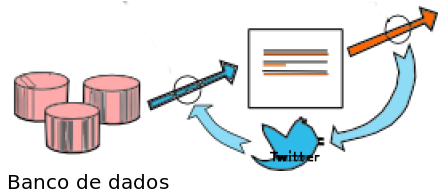
\includegraphics[width=90mm, height=45mm]{Figuras/Metodologia/ArcoCibernetico.png}\\
\tiny Fonte: autor
\end{figure}



\section{Extrapolação para georreferenciamento}

\pagebreak
